\documentclass[ExampleMasters.tex]{subfiles}
\begin{document}

	\chapter{APPENDIX E}
	{\Large Battery degradation and replacement}

	\section{Factors affecting battery life}
		The amount of active battery electrolytes reacting to produce electric potential is dependent on a host of parameters such as the electrolyte temperature, battery current, depth of discharge and charging/discharging rates. Cell ageing also adversely affects battery performance apart from passive factors such as mechanical stresses, passivation of electrodes etc.\\

		In this thesis, the effect of the battery depth of discharge is considered to estimate a working lifetime of the battery, based on which the number of battery replacements during the lifetime of the vehicle can be calculated.\\

	\section{Effect of depth of discharge}
		The amount of chemicals that react depends directly on the depth of discharge. It is observed that with increasing depth of discharge, the number of charge-discharge cycles that a battery can survive falls logarithmically \cite{BatteryLife}. Drouilhet \textit{et al} provide a logarithmic relationship between battery life, $L$, in number of lifetime charge-discharge cycles and depth of discharge, $D$, in \cite{BatteryLifeDoDRelation} as shown below:

		\begin{equation}
			L_{batt, D} = u_2 \left(\frac{D_R}{D}\right)^{u_0} e^{u_1\left(1-\frac{D}{D_R}\right)}
		\end{equation}

		\nomenclature{$L_{batt, D}$}{Battery lifetime in number of charge-discharge cycles (cycles)}
		\nomenclature{$u_i$}{Equation constants in battery - DoD relation}	
		\nomenclature{$D_R$}{Depth of Discharge for which rated cycle life is determined (\%)}
		\nomenclature{$D$}{Actual maximum depth of discharge (\%)}

		For the chosen brand of batteries, the number of lifetime cycles yielded at 100\% depth of discharge is 1000 and the lifetime yielded at 20\% depth of discharge is 100000. These data points are fitted to the above relation while choosing the lifetime at 20\% DoD as the rate cycle life, $D_R$. The fitted relation is:

		\begin{equation}
			L_{batt, D} = 100000 \left(\frac{D_R}{D}\right)^{0.376} e^{\left(1-\frac{D}{D_R}\right)}
			\label{BattLifeDoD}
		\end{equation}

		\begin{figure}[ht!]
			\centering
			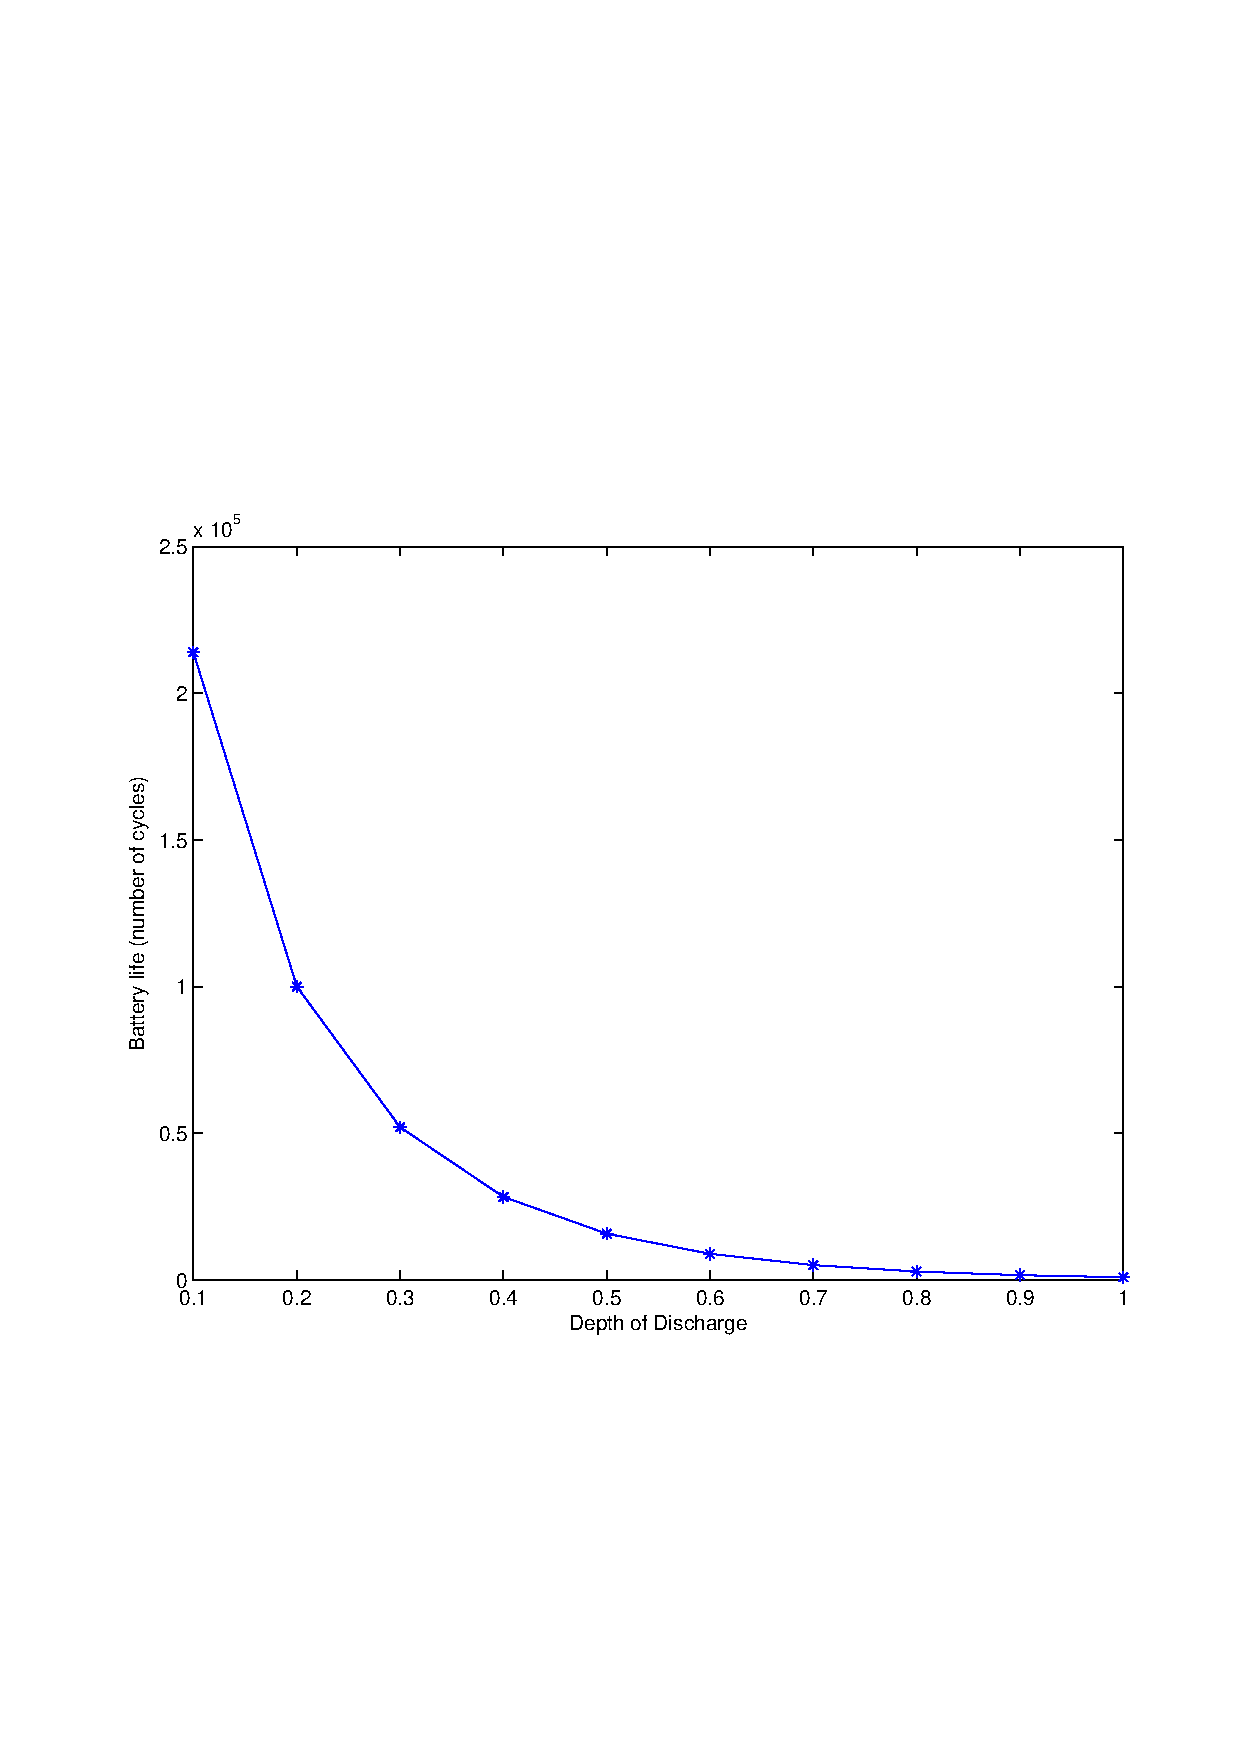
\includegraphics[width=0.5\textwidth, clip=true, trim=60 185 45 245]{figures/Appendices/BatteryLifeVsDoD.pdf}
			\caption{Battery life-cycles vs Cycle Depth of Discharge}
			\label{BattLifeVsDoD}
		\end{figure}

	\section{Battery replacements}
		For every mission, the maximum achieved depth of discharge $D_{max}$ is used in Equation \eqref{BattLifeDoD} to calculate the lifetime of the battery $L_{batt, D_{max}}$. 

		\begin{equation}
			L_{batt, D_{max}} = 100000 \left(\frac{D_R}{D_{max}}\right)^{0.376} e^{\left(1-\frac{D_{max}}{D_R}\right)}
		\end{equation}

		The number of charge-discharge cycles $N_{ch/disch}$ to maximum depth of discharge is calculated at the end of each mission. \nomenclature{$N_{ch/disch}$}{Number of charge-discharge cycles to maximum depth of discharge (cycles)} If the number of daily missions is $N_{mission, daily}$ \nomenclature{$N_{mission, daily}$}{Number of daily missions}, the number of times the battery will have to replaced during the lifetime of the vehicle (first-owner) is given by

		\begin{equation}
			N_{batt, replacement} = \frac{Total\  number \ of \ battery\  charge-discharge \ cycles\  over\  vehicle \ lifetime}{Number\  of\  charge-discharge\  cycles\  over \ a \ single\  battery\  lifetime}
		\end{equation}
		
		or,

		\begin{equation}
			N_{batt, replacement} = \frac{N_{mission, daily} \times 365 \times N_{first\ owner} \times N_{ch/disch}}{L_{batt, D_{max}}}
		\end{equation}

		Thus, while calculating mission productivity over $N_{first\ owner}$ years, the battery costs are compounded by the number of replacements during the $N_{first\ owner}$ years. The higher the depth of discharge, the lower the battery lifetime. As a result, battery use can be maximised at the cost of increased battery replacements.\\

	\newpage
\end{document}